After the software was adapted to the physical drone systems, a large WhyCon marker was printed as a landing pad, as shown in Figure \ref{fig:landing_pad}. It was then attached to a piece of plexiglass for rigidity. The paper unfortunately does get dirty and absorbs moisture and must therefore be replaced from time to time. This method reduces glossiness and glare on the landing platform, and provides exactitude in the shape of the marker, as opposed to painting the marker by hand.

\begin{figure}
    \centering
    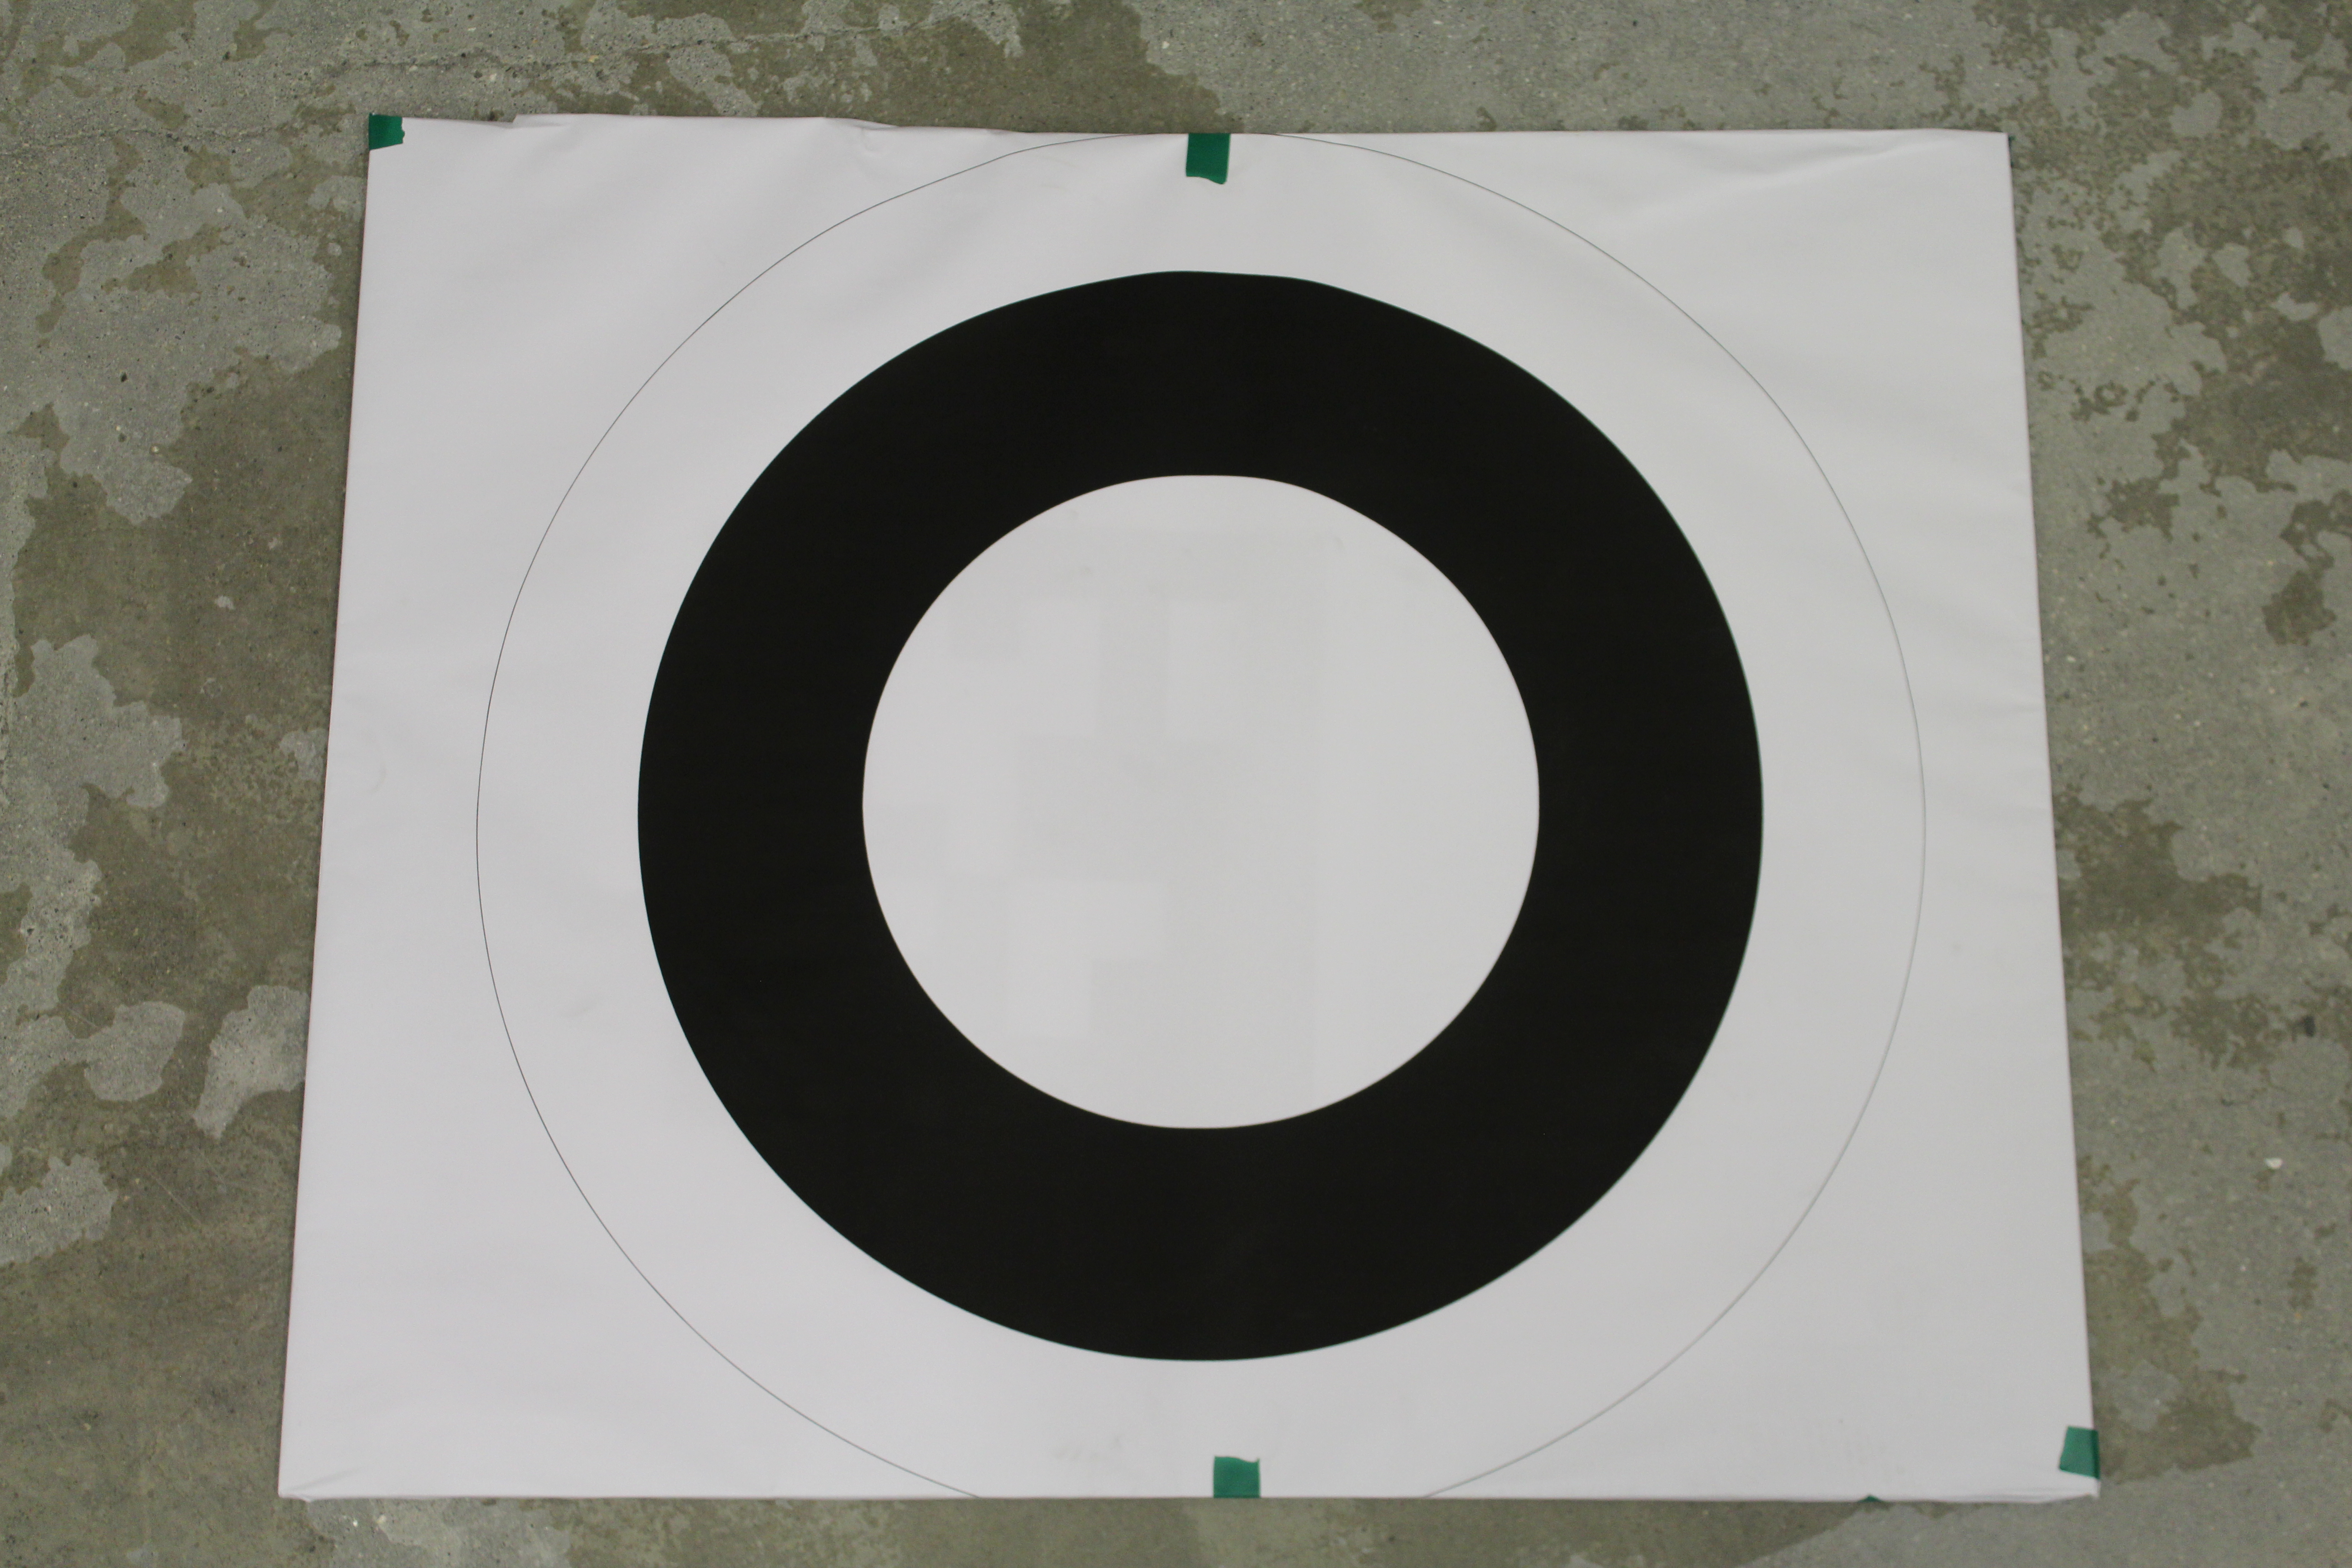
\includegraphics[width=0.5\textwidth]{images/landing_pad.JPG}
    \caption{The landing pad.}
    \label{fig:landing_pad}
\end{figure}